% !TEX encoding = UTF-8 Unicode
\documentclass[10pt, a4paper]{article}

\usepackage{amsmath}
\usepackage{footnote}
\makesavenoteenv{tabular}
\usepackage{ltc05}
%\usepackage{polski}
\usepackage[utf8]{inputenc}
\usepackage{textcomp} 
\usepackage[T1]{fontenc}
\usepackage{lmodern}
\usepackage{url}
\usepackage{graphicx}
\title{A Sequential Child Combination Tree-LSTM Network for Sentiment Analysis}


%%%%%%%%%%%%%%%%%%%%%%%%%%%%%%%%%%%%%%%%%%%%%%%%%%%%%%%%%%%%%%%%%%%%%%%%%
%!!!!!!!!!!!!!!!!!!!!!!!!!!!!!!!!!!!!!!!!!!!!!!!!!!!!!!!!!!!!!!!!!!!!!!!!
%!!!!!!!!!!!!!!!!!!!!!!!!!!!!!!!!!!!!!!!!!!!!!!!!!!!!!!!!!!!!!!!!!!!!!!!!
% PLEASE DO NOT WRITE YOUR NAME AND ADDRESS IN THE DRAFT OF YOUR PAPER
% SIMPLY ERASE THE LINES...
\name{Michał Lew$^{\dagger}$\\ \bf \large Piotr Pęzik$^{\ast}$} 

\address{ $^{\dagger}$VoiceLab \\	
               michal.lew@voicelab.pl \\ \\
               $^{\ast}$University of Lodz \\ 
               piotr.pezik@uni.lodz.pl}

%% ... UP TO HERE
% ... UP TO HERE
%!!!!!!!!!!!!!!!!!!!!!!!!!!!!!!!!!!!!!!!!!!!!!!!!!!!!!!!!!!!!!!!!!!!!!!!!
%!!!!!!!!!!!!!!!!!!!!!!!!!!!!!!!!!!!!!!!!!!!!!!!!!!!!!!!!!!!!!!!!!!!!!!!!
%%%%%%%%%%%%%%%%%%%%%%%%%%%%%%%%%%%%%%%%%%%%%%%%%%%%%%%%%%%%%%%%%%%%%%%%%


\abstract{This paper describes a sentiment analysis system submitted to the PolEval 2017 competition.}

\begin{document}

\maketitleabstract

\section{Introduction}   
Sentiment Analysis (SA) is an active area of natural language processing research with applications in marketing research, customer relations management systems, social media communication studies to mention just a few examples. A common objective of SA is to automatically detect the attitudinal value of an utterance or otherwise coherent stretch of text which can be attributed to a particular author. The distribution of  such attitudinal values in an utterance is usually known as its \textit{polarity} and it usually ranges from positive to neutral and negative \cite{cambria_schuller}, possibly with finer-grained distinctions between these main categories, such as \textit{somewhat positive} or \textit{very negative} \cite{socher2013recursive}. More recent approaches to SA focus on phrase-level polarity classification, whereby attitudinal or emotional values are detected at the level of syntactic phrases and only then compositionally combined to compute the polarity of an entire utterance. Such approaches are particularly important in aspect-based SA, where different aspects of one's opinion about a product, movie, person, etc. have to be detected in addition to  classifying the overall sentiment of a text unit. Also, phrase-level models of SA are better suited to deal with basic syntactic phenomena such as negation or modality, which may cause a significant shift in the predominant sentiment of an utterance \cite{wilson_wiebe}. 
\par The present paper evaluates a deep-learning based system for syntax-driven SA, which was submitted to the PolEval 2017 competition. We first briefly describe the syntactically annotated sentiment datasets used and the nature of the classification task. Next, we present the Sequential Child-Combination Tree-LSTM Network model used to implement the proposed system and evaluate its performance on the PolEval test set.


\section{PolEval 2017}

The dataset released in the PolEval competition for the task described in this paper can be described as a sentiment dependency treebank. In general, sentiment treebanks are collections of syntactically parsed sentences which have sentiment annotations assigned to their constituent words or phrases. The type of sub-sentential word combinations which are annotated with  sentiment labels may depend on the exact syntactic formalism used in a given treebank. For example, the Stanford Sentiment Treebank \cite{socher2013recursive} contains full (binary) constituency parse trees comprising phrases associated with five sentiment classes. On the other hand, the sentences in the PolEval dataset, are dependency-parsed. As we explain below, this has implications for modelling an SA system which makes use of syntactic annotations. For example, unlike the above-mentioned constituency representations, most sentence dependency graphs are N-ary trees in that a word node may directly govern only one or more than two other word vertices as shown in \ref{fig:dep_sent}, where the verb \textit{drażni} has four direct dependents, and the noun \textit{dniu} has only one dependent adjective \textit{całym}. 
\par This example sentence\footnote{Its word-for-word into English could be \textit{(It) doesn't irritate even after a whole day.}} also illustrates the point of using syntactic annotation in sentiment analysis. It is quite evident that it expresses a customer's overall satisfaction with a particular brand of perfume, even though its (directly negated) main verb \textit{drażnić} (irritate) could be found in a list of keywords denoting negative sentiment. On a more subtle level, the positive attitude of this utterance towards this particular product is further reinforced by the indirectly negated adverbial clause (i.e. \textit{even after a whole day}), which denotes a condition in which other fragrances might be irritating.
\par Table \ref{tab:nie_drazni_1} illustrates the type of annotations made available in the PolEval 2017 sentiment analysis datasets. For each word in a sentence (listed in row \texttt{W}) its parent word node was indicated (see row \texttt{P}) together with its sentiment label (as in row \texttt{S}). The parent labels could be used to reconstruct the syntactic dependency tree of this sentence as shown in Fig. \ref{fig:dep_sent}. The goal of the SA subtask was to  a) correctly identify sentiment labels of each leaf word node and b) to correctly predict the sentiment label of every complete subtree starting in every non-terminal node of the sentence tree. The list of such leaf nodes and subtrees for which sentiment labels would have to be detected if the example sentence was found in the test set is shown in Table \ref{tab:nie_drazni_2}. The overall sentiment of an utterance is thus predicted from the sentiment value of its root node, which is usually the main verb of a sentence and the subtrees of the dependency trees considered in this task (other than the terminal word nodes) are always complete constituency phrases. 
\begin{table}[h]
 \begin{center}
\begin{tabular}{|l| l l l l l l l|}
      \hline
      %Level&Tools\\
      %\hline\hline
      W & Nie & drażni & nawet & po & całym & dniu & . \\
      \hline
      P & 2 & 0 & 2 & 2 & 6 & 4 & 2 \\
      \hline
      S & 0 & 1 & 0 & 0 & 0 & 0 & 0 \\
      \hline
\end{tabular}
\caption{An example PolEval dataset sentence with phrase-level sentiment annotation (W -- word nodes, P -- syntactic parents, S -- polarity value).}
\label{tab:nie_drazni_1}
 \end{center}
\end{table}



\begin{figure}
  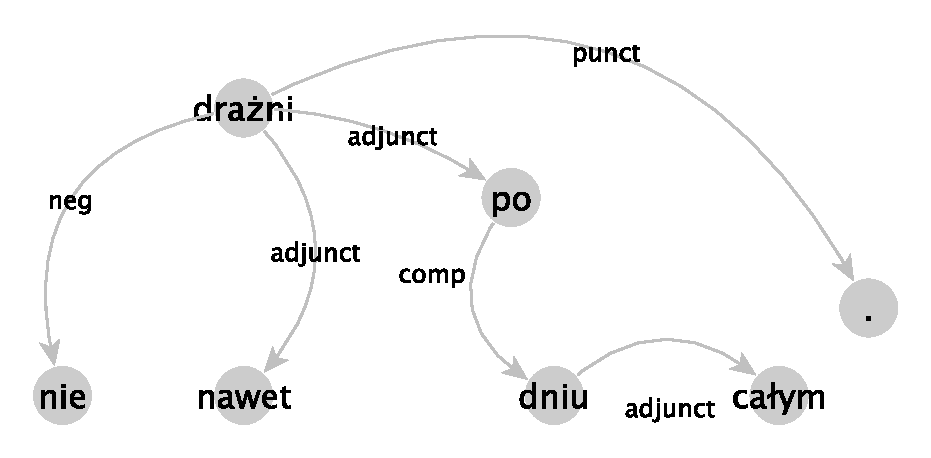
\includegraphics[width=\linewidth]{imgs/nie_drazni.pdf}
  \caption{A dependency representation of the example sentence shown in Table \ref{tab:nie_drazni_1}.}
  \label{fig:dep_sent}
\end{figure}

\begin{table}[h]
 \begin{center}
\begin{tabular}{|l | l|}

\hline
 Word &	Polarity\\
      \hline
     Nie &	0\\
     \hline
Nie drażni nawet po całym dniu	 . & 1\\
\hline
nawet &	0\\
\hline
po całym dniu &	0\\
\hline
całym dniu &	0\\
\hline
.	& 0\\
      \hline
\end{tabular}
\caption{Phrase- and word-level sentiment values to be predicted for the example sentence shown in Table \ref{tab:nie_drazni_1}.}
\label{tab:nie_drazni_2}
 \end{center}
\end{table}

\section{Model} 


\subsection{LSTM Neural Networks}

Different variants of Recurrent Neural Networks (RNNs) have been widely used for many task in natural language processing such named entity recognition \cite{lample2016neural} or text classification \cite{lai2015recurrent}. They can process the arbitrarily long inputs by recurrent application of a transition function over hidden states. The most common form of an RNN transition function is an affine transformation followed by a hyperbolic tangent function:
	\begin{equation} h_t = tanh(W_{x_t}+U_{h_{t-1}}+b)
\end{equation}
	A potential advantage of RNNs in processing natural language stems from their ability to use information gathered sequentially from previous states, such as words or phrases. In theory this makes them capable of tracking a long history of previous states when processing sequences of words. In practice, however, RNNs may they suffer from so-called vanishing gradient problem, which means that during training the gradient can grow or decay exponentially over long sequences \cite{bengio1994learning,hochreiter1998vanishing}. The LSTM architecture \cite{hochreiter1997long} addresses the problem of learning long-term dependencies by introducing a memory cell that is capable of preserving previous state information over relatively long sequences of state. [citation]
\par There are many different variants of LSTMs, in our work we used following equations:
		
\begin{equation}
\begin{split}
		&i_t = \sigma(U^i{x_t} + W^is_{t-1} + b^i) ,\\
		&f_t = \sigma(U^f{x_t} + W^fs_{t-1} + b^f) ,\\
		&o_t = \sigma(U^o{x_t} + W^os_{t-1} + b^o) ,\\
		&g_t = \tanh(U^g{x_t}+ W^gs_{t-1} + b^g) ,\\
		&c_t = c_{t-1} \bullet f_t + g_t \bullet i_t ,\\
		&s_t = \tanh(c_t) \bullet o_t 
\end{split}
\end{equation}

		where $x_t$ is input at current time step, $i_t$ is an input gate, $f_t$ a forget gate, $o_t$ an output gate and $c$ stands for LSTM memory.
		The gates mechanism controls how much information from past states and memory is used at the current time step. 

\subsection{Tree-LSTM}
\begin{figure}[h]
	\begin{center}
		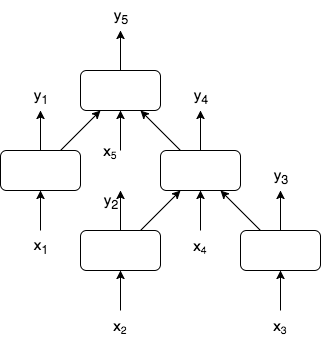
\includegraphics[width=0.3\textwidth]{imgs/tree-lstm}
		\caption{A Tree-LSTM architecture's structure}
		\label{tab:tree-lstm}
	\end{center}
\end{figure}
	The problem with classical LSTM's is as with the standard RNNs that they are linear chain which makes them useless for processing more sophisticated structures than sequences. In particular, many linguistic beings are represented with tree-structure [citation? jakiś Chomsky czy coś fajnego :D].
	In order to process tree-structured data we need to extend the LSTM architecture. In case of such structures as trees the model architecture called Tree-LSTM was introduced \cite{tai2015improved}.
	In general, tree-structured Recurrent Neural Networks expand basic RNNs by creating a way to plug in more than one previous state to hidden unit at given time step as shown at Figure 2.
	Each unit takes an input $x_j$ and emits label $y_j$ as in standard RNN. However, here each unit can take more than one previous hidden state. Tree-LSTM in particular add the memory to that architecture.
	
\subsection{Tree-LSTM label classification}
		In our case we are dealing with sentences represented as trees. That means each $x_j$ is a word represented as vector called Word Embedding
		[citation  Mikolov, Tomas; Sutskever, Ilya; Chen, Kai; Corrado, Greg; Dean, Jeffrey (2013). "Distributed Representations of Words and Phrases and their Compositionality". arXiv:1310.4546 Freely accessible [cs.CL].]. If the network unit is a leaf, than its hidden state is an embedding of its word input. If the network unit is not a leaf however, its hidden state represents embedding of entire subtree it represents. That means, if we compute softmax function of that hidden state we will receive label for entire subtree, in our case sentiment label. From it follows that hidden state of root unit is the embedding of entire sentence and its label is the label of entire sentence.\\
	\indent
	
	There can be different types of Tree-LSTM architecture depending on tha way in which child units are incorporated into its parent unit. In our work we show Child-Sum Tree-LSTM architecture \cite{tai2015improved} and present new Sequential-Child-Combination Tree-LSTM architecture.\\
\subsection{Child-Sum Tree-LSTM}

 For dealing specificly with dependency trees the Child-Sum Tree-LSTM model was presented \cite{tai2015improved}. Its transition equations are the follwing:
\begin{equation}
\begin{split}
&s_{ch}=\sum_{k}s_{ch_k},\\
&i_j = \sigma(U^ix_j + W^is_{ch} + b^i) ,\\
&f_{jk} = \sigma(U^fx_j + W^fs_{ch_k} + b^f) ,\\
&o_j = \sigma(U^ox_j + W^os_{ch} + b^o) ,\\
&g_j = \tanh(U^gx_j+ W^gs_{ch} + b^g) ,\\
&c_j = \sum_{k} c_k \bullet f_{jk} + g_{j} \bullet i_{j} ,\\
&s_j = \tanh({c_{j}}) \bullet o_{j},\\
\end{split}
\end{equation}
	where $k$ is a subscript of $k$-th child of node $j$ and $s_{ch_k}$ is its hidden state.
\subsection{Sequential-Child-Combination Tree-LSTM}

\begin{figure}[h]
	 \begin{center}
    	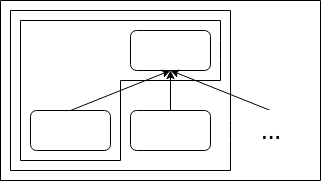
\includegraphics[width=0.3\textwidth]{imgs/sequentialchild}
		\caption{Sequentially combining the children with parent}
		\label{tab:sequentialchild}
	 \end{center}
\end{figure}
	In our work we we propose the Sequential-Child-Combination Tree-LSTM architecture. We combine children with its parent as follows:
\begin{equation}
\begin{split}
&i_{i_1} = \sigma(U^i{x_t} + W^i{s_{ch_1}} + b^i) ,\\
&f_{i_1} = \sigma(U^f{x_t} + W^f{s_{ch_1}} + b^f) ,\\
&o_{i_1} = \sigma(U^o{x_t} + W^o{s_{ch_1}} + b^o) ,\\
&g_{i_1} = \tanh(U^g{x_t}+ W^g{s_{ch_1}} + b^g) ,\\
&c_{i_1} = c_{t-1} \bullet f_{i_1} + g_{i_1} \bullet i_{i_1} ,\\
&s_{i_1} = \tanh({c_{i_1}}) \bullet o_{i_1},\\\\
&i_{i_2} = \sigma(U^is_{i_1} + W^is_{ch_2} + b^i) ,\\
&f_{i_2} = \sigma(U^fs_{i_1} + W^fs_{ch_2} + b^f) ,\\
&o_{i_2} = \sigma(U^os_{i_1} + W^os_{ch_2} + b^o) ,\\
&g_{i_2} = \tanh(U^gs_{i_1}+ W^gs_{ch_1} + b^g) ,\\
&c_{i_2} = c_{i_1} \bullet f_{i_2} + g_{i_2} \bullet i_{i_2} ,\\
&s_{i_2} = \tanh(c_{i_2}) \bullet o_{i_2},\\\\
&\cdots\\\\
&i_{i_n} = \sigma(U^is_{{n-1}} + W^is_{ch_{n}} + b^i) ,\\
&f_{i_n} = \sigma(U^fs_{{n-1}} + W^fs_{ch_{n}} + b^f) ,\\
&o_{i_n} = \sigma(U^os_{{n-1}} + W^os_{ch_{n}} + b^o) ,\\
&g_{i_n} = \tanh(U^gs_{{n-1}}+ W^gs_{ch_{n}} + b^g) ,\\
&c_{i_n} = c_{i_{n-1}} \bullet f_{i_n} + g_{i_n} \bullet i_{i_n} ,\\
&s_{i_n} = \tanh(c_{i_n}) \bullet o_{i_n},\\\\
&c_{t} = c_{i_n}\\
&s_{j} = s_{i_n}
\end{split}
\end{equation}
	where $s_{i_k}$ is an intermediate state after combining with $k$-th children. That means, we can see each Tree-LSTM unit as linear LSTM chain dealing with each child respectively. $c$ is a one global memory updated lineary.
	Despite the fact that in dependency tree the children are unordered this way of combining them allows for creating the embeddings made of subphrases of particular children and remember that, which is not possible in case of Child-Sum Tree-LSTM. Moreover, same order can be introduced by taking firstly the children that are earlier in sentence order. With that we are able to use the relation between father and particular children in potentially deeper way that with Child-Sum Tree-LSTM.\\
	%Pomimo, że w drzewie zależnościowym dzieci nie są ułorzone wg porządku takie działanie pozwala na tworzenie zanurzeń fraz tworzonych z poszczególnych dzieci i %zapamiętywanie ich, co nie jest możliwe w przypadku Child-Sum Tree-LSTM. Ponadto, pewien porządek można nadać poprzez branie najpierw dzieci będących wcześniej w %szyku zdaniowym. W ten sposób jesteśmy w stanie w potencjalnie głębszy sposób wykorzystać relacje pomiędzy ojcem a poszczególnymi dziećmi niż w przypadku Child-Sum %Tree-LSTM.\\
\indent
Intuitively, we combine parent with its children in a way that we create intermidiate embeddings by combining child phrases with continuously updated parent phrase. That means we firstly combine parent with its first child which is a subtree with root at that node, then we combine result with next child-subtree and so on. Final state after combining all children creates embedding of entire phrase. This is shown at Fig. \ref{tab:sequentialchild} and example is given at Fig. \ref{tab:niedrazniex}.\\
\indent
	Also, it is possible to manage the memory in a different way than presented. We experimented with using separate memory for each unit but eventualy the best results were obtained using the presented method.

%Intuicyjnie, łączymy dzieci z rodzicem od lewej do prawej w taki sposób, że tworzymy pośrednie zanurzenia niosące informację o ojcu uzupełnioną o informację o poddrzewie, którego korzeniem jest dane dziecko.
%Ostateczny stan po połączeniu ze wszystkimi dziećmi tworzy znaczenie całego drzewa.
%Przykład 'Stary rudy kot wlazł na płot'
%mamy kot-stary kot-rudy kot-wlazł
%z tego wychodzi, że stary kot-rudy stary kot-wlazł
%stary rudy kot-wlazł itd.
%można przedstawić taki przykład, żeby pokazać intuicję stojącą za tym sposobem.
\begin{figure}[h]
	\begin{center}
		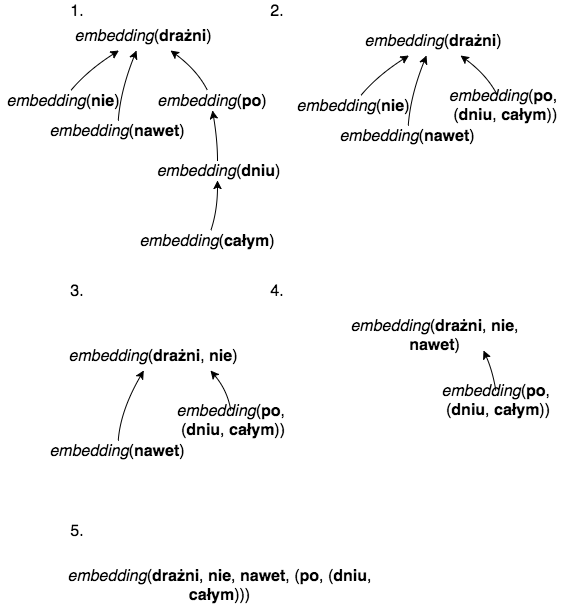
\includegraphics[width=0.5\textwidth]{imgs/niedrazniex}
		\caption{Example of combining children with its parent.}
		\label{tab:niedrazniex}
	\end{center}
\end{figure}
	
\section{Evaluation} 
	We compare our results with mentioned Child-Sum Tree-LSTM, simple linear-chain LSTM and Conditional Random Fields (CRF).  Results are shown in Table \ref{tab:evaluation}.
	[co z lematyzacją, jak to opisać?]
\begin{table}[h]
 \begin{center}
\begin{tabular}{|l|l|}

      \hline
      %Level&Tools\\
      %\hline\hline
      Model & Score\\
      \hline
      LSTM &70,70\%\\
      \hline
      Lemmatized CRF & 75,63\%\\
      \hline
      Child-Sum Tree-LSTM &  77,69\%\\
      \hline
      Sequential-Child-Combination Tree-LSTM & 78,56\%\\
      \hline
      Lemmatized Child-Sum Tree-LSTM & 78,90\%\\
      \hline
      Lemmatized Sequential Child Combination & \\
      Tree-LSTM & \textbf{79,89\%} \\
      \hline
\end{tabular}
\caption{Sentiment classification accuracy on the PolEval test set.}
\label{tab:evaluation}
 \end{center}
\end{table}



\section{Conclusions and future work}


\section{Availability}

The source code of the system described in this paper, together with the trained models, datasets are available at \url{https://githubXXX}.

%\nocite{*}

\section{Acknowledgments}

\bibliographystyle{ltc05}
\bibliography{sal} 

\end{document}

